\documentclass{article}
\usepackage[T1]{fontenc}
\usepackage{lmodern}
\usepackage{graphicx}
\usepackage{amsmath,amssymb}
\usepackage[a4paper,margin=2cm]{geometry}
\usepackage[absolute,overlay]{textpos}
\setlength{\TPHorizModule}{1mm}
\setlength{\TPVertModule}{1mm}
\usepackage[indonesian]{babel}
\usepackage{hyperref}
\setlength{\emergencystretch}{2em}
% unit: Halaman 114

\begin{document}

% === Halaman 114 (python/native) ===

114

• Posisi awal keempat rotor dapat di-set; dan posisi 

awal ini menyatakan kunci dari Enigma. 

• Kriptanalisis 

mesin 

Enigma 

pertama 

kali 

ditemukan pada tahun 1932 oleh kriptografer 

Polandia, yaitu Marian Rejewski, Jerzy Różycki 

dan Henryk Zygalski.

• Pemerintahan Nazi Jerman kemudian mendesain 

ulang mesin Enigma pada tahun 1939  dengan 

menambahkan 

plugboard 

dan 

refelector, 

sehingga proses enkripsi menjadi lebih kompleks. 

Metode kriptanalisis Enigma sebelumnya tidak 

dapat digunakan lagi.

% deskripsi: gambar native xref 409
\noindent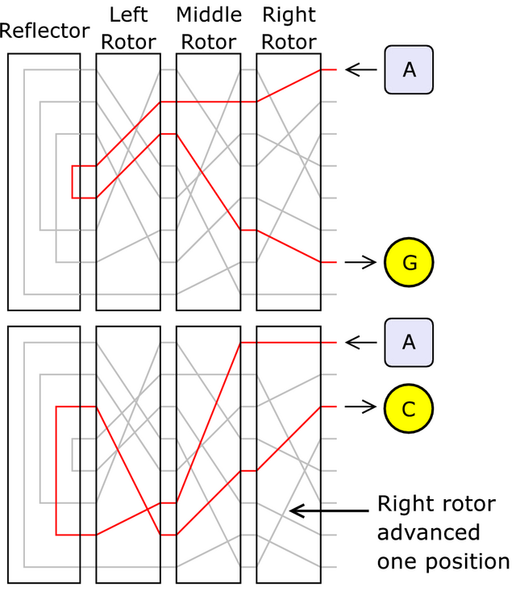
\includegraphics[width=0.85\textwidth]{../../images/python/page_114_img_01.png}

\end{document}
